% !TEX TS-program = pdflatex
% !TEX encoding = UTF-8 Unicode

% This is a simple template for a LaTeX document using the "article" class.
% See "book", "report", "letter" for other types of document.

\documentclass[11pt, french]{article} % use larger type; default would be 10pt
\usepackage[francais]{babel}
\usepackage[utf8]{inputenc} % set input encoding (not needed with XeLaTeX)
\usepackage[T1]{fontenc}
\usepackage[squaren,Gray]{SIunits}
\usepackage{amsmath}
\usepackage{hyperref}
%%% Examples of Article customizations
% These packages are optional, depending whether you want the features they provide.
% See the LaTeX Companion or other references for full information.

%%% PAGE DIMENSIONS
\usepackage{geometry} % to change the page dimensions
\geometry{a4paper} % or letterpaper (US) or a5paper or....
% \geometry{margin=2in} % for example, change the margins to 2 inches all round
% \geometry{landscape} % set up the page for landscape
%   read geometry.pdf for detailed page layout information

\usepackage{graphicx} % support the \includegraphics command and options

% \usepackage[parfill]{parskip} % Activate to begin paragraphs with an empty line rather than an indent

%%% PACKAGES
\usepackage{booktabs} % for much better looking tables
\usepackage{array} % for better arrays (eg matrices) in maths
\usepackage{paralist} % very flexible & customisable lists (eg. enumerate/itemize, etc.)
\usepackage{verbatim} % adds environment for commenting out blocks of text & for better verbatim
\usepackage{subfig} % make it possible to include more than one captioned figure/table in a single float
% These packages are all incorporated in the memoir class to one degree or another...

%%% HEADERS & FOOTERS
\usepackage{fancyhdr} % This should be set AFTER setting up the page geometry
\pagestyle{fancy} % options: empty , plain , fancy
\renewcommand{\headrulewidth}{0pt} % customise the layout...
\lhead{}\chead{}\rhead{}
\lfoot{}\cfoot{\thepage}\rfoot{}

%%% SECTION TITLE APPEARANCE
\usepackage{sectsty}
\allsectionsfont{\sffamily\mdseries\upshape} % (See the fntguide.pdf for font help)
% (This matches ConTeXt defaults)

%%% ToC (table of contents) APPEARANCE
\usepackage[nottoc,notlof,notlot]{tocbibind} % Put the bibliography in the ToC
\usepackage[titles,subfigure]{tocloft} % Alter the style of the Table of Contents
\renewcommand{\cftsecfont}{\rmfamily\mdseries\upshape}
\renewcommand{\cftsecpagefont}{\rmfamily\mdseries\upshape} % No bold!

%%% END Article customizations

%%% The "real" document content comes below...

\title{TP1 - IFT2015\\- Analyse -}
\author{Tristan Savaria}
\date{9 février 2014} 

\begin{document}
\maketitle
\newpage
\tableofcontents
\newpage
\section{Résultats et Conclusion}
\paragraph{}

\subsection{Insertion}

\begin{figure}[htbp]
\centering
\fbox{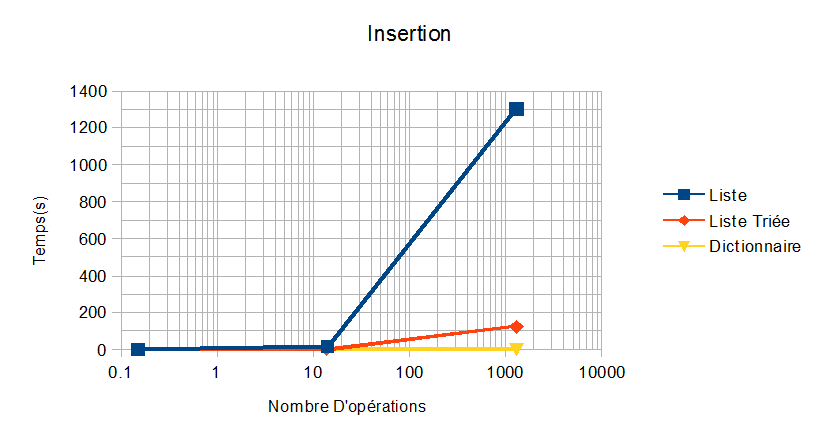
\includegraphics[width=\textwidth]{insertion.png}}
\end{figure}
On observe que l'insertion dans la structure de Liste consomme beaucoup plus de temps que les deux autres structures. Une liste ajoute habituellement un élément dans l'ordre de O(1). 
Cependant, dans le cadre de ce projet, chaque insertion requiert une recherche pour trouver si le Mot y est déjà présent pour incrémenter son compte si c'est le cas. La recherche pour la liste est dans l'ordre de O(n) et c'est pour cela que l'insertion dans la structure de Liste est aussi lente.
\newline
La liste triée arrive seconde puisqu'à chaque insertion une recherche binaire est effectué pour insérérer/trouver l'élément au bon index.

\subsection{Recherche}
\begin{figure}[htbp]
\centering
\fbox{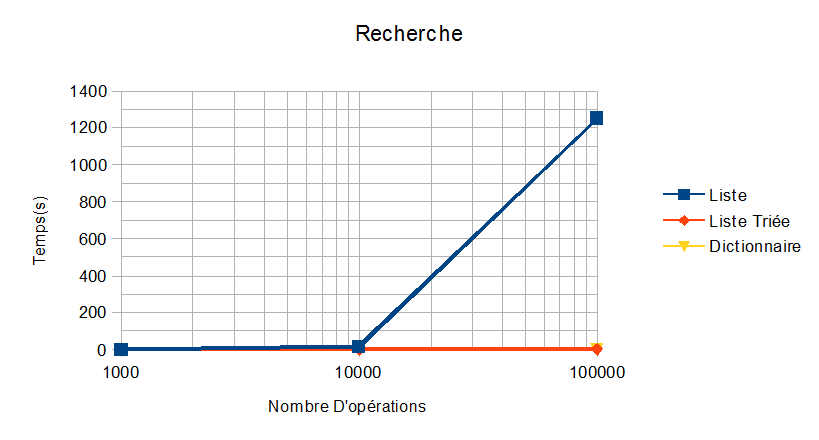
\includegraphics[width=\textwidth]{recherche.png}}
\end{figure}
La recherche dans la structure liste est la plus lente, car au pire cas nous devons comparé chaque élément de la liste à celui que nous cherchons ce qui est dans l'ordre O(n).
Liste Triée et Dictionnaire sont confondues par une erreur de formatage de ma part, cependant Dictionnaire est plus rapide avec 0.04 sec pour 100 000 opérations contre 2.64 sec pour la Liste Triée. Liste Triée utilise une recherche binaire, cependant le hashtable de dictionnaire est plus rapide.
\newline

\subsection{Suppression}
\begin{figure}[htbp]
\centering
\fbox{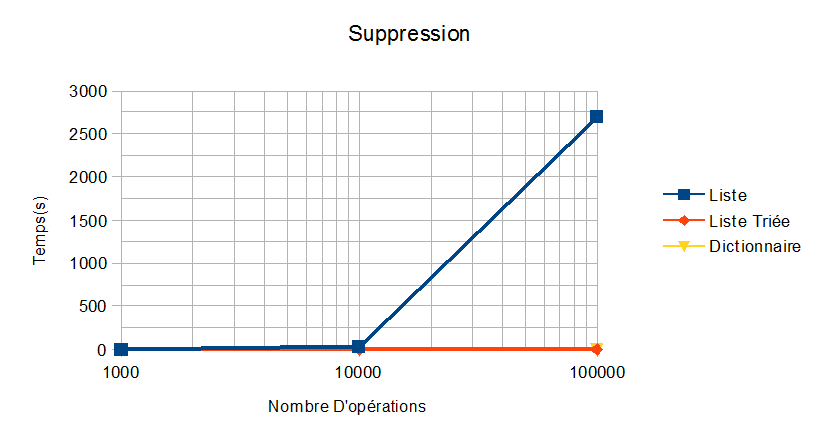
\includegraphics[width=\textwidth]{suppression.png}}
\end{figure}
La suppression est plus lente pour la Liste. Comme pour l'insertion, une recherche est effectué sur la structure pour trouver l'élément à supprimer. 
Liste Triée et Dictionnaire sont confondues par une erreur de formatage de ma part, cependant Dictionnaire est plus rapide avec 0.07 sec pour 100 000 opérations contre 2.54 sec pour la Liste.
Nous pouvons observer que la suppression a été aussi rapide que la recherche pour la Liste Triée et le dictionnaire.


\section{Commentaire}
Il est possible que le code que j'ai utilisé pour la prise de mesure a eu un impact sur la validité des données. Par example, le code utilisé ne générait pas le cas ou l'élément à rechercher et à supprimer n'existait pas dans la structure. La structure de liste est capable de mieux performer dans le cas de l'insertion s'il était possible de ne pas faire de recherche avant l'insertion. Cependant, par la nature de ce travail il est impossible de contourner cette restriction. Avec plus d'éléments il serait possible d'observer le cas ou la Liste Triée et le Dictionnaire ne sont plus confondue en une seule ligne.
\newline

\end{document}
